\documentclass[10pt]{article}
\usepackage[margin=0.85in]{geometry}
\usepackage{amsmath,amssymb}
\usepackage[T1]{fontenc}
\usepackage[utf8]{inputenc}
\usepackage{lmodern}
\usepackage{microtype}
\usepackage{booktabs}
\usepackage{enumitem}
\usepackage{graphicx}
\usepackage[hidelinks]{hyperref}
\hypersetup{pdftitle={Where Does Cold Dark Energy Switch On?}}
\setlist{nosep,leftmargin=1.3em}
\setlength{\parskip}{3pt}\setlength{\parindent}{0pt}
\sloppy
\begin{document}
\begin{center}
{\Large\bfseries Where Does Cold Dark Energy Switch On?\\ A Precisely Posed Question at $M\gtrsim10^{12.4}\,M_\odot$}\\[6pt]
{\small Working note, 2026-10-27, v1.0 (draft 1). AI-assisted research programme; not peer reviewed. $\kappa=\tfrac12$ is fitted; the theory is not closed.}
\end{center}

\begin{abstract}\noindent
The programme studies a galaxy law, $g_N=g^2/(g+a_0)$ with $a_0=c^2\sqrt{\Lambda/32\pi}$ ($\kappa=\tfrac12$ fitted), together with a gravitating $w\approx0$ field component, called here \emph{cold dark energy} (not matter, not a particle). The law fits isolated galaxies; groups and clusters need cold dark energy halos. The record's best organising rule is environment-keyed: cold dark energy halos in satellites and in systems above a mass threshold; the law on baryons alone below it. This note does not claim a mechanism. It states, from frozen and reproduced calculations, \emph{what the mechanism must do}:
\begin{enumerate}
\item \textbf{The threshold is not the core-floor crossover.} If the threshold is X43's crossover $\eta\,\Sigma_{\rm coll}(M)=a_0/2\pi G$ (with $\eta\propto c_f^{5/4}$), one number $c_f$ sets both where condensation starts and how concentrated group and cluster cores are. On a grid $c_f=3.5$--$6.0$ no value passes every graded line (CF1). KiDS isolated-lens lensing passes only at $c_f=3.5$, i.e. a threshold $\ge10^{12.39}\,M_\odot$ (canonical footing); groups pass only for $c_f\ge4.75$ on both footings, which lowers the threshold below $10^{11.72}$.
\item \textbf{Cluster outskirts and cluster centres pull $c_f$ apart.} The outskirts of the most gas-rich clusters pass only for $c_f\ge5.25$; the inner band of all 326 clusters passes only for $c_f\le5.0$. One cored profile cannot do both.
\item \textbf{The outskirt deficit is not correlated structure beyond turnaround} (GC1): that mass projects as a nearly flat sheet and changes the outer predictions by at most 1.3\,\%.
\item \textbf{Below the threshold}, the surviving exclusion mechanism (M6, initial displacement) is not yet tested by the Lyman-$\alpha$ forest: four native forest models of increasing fidelity are each not diagnostic. If the forest-side budget is real, galaxies needing M6 must keep at least 19--56\,\% (canonical) or 28--83\,\% (alternative) of their initial patch baryons, against the record's own Lagrangian retention of 19.1\,\% / 16.3\,\%.
\end{enumerate}
\textbf{The question posed:} what physics switches cold dark energy on at $M\gtrsim10^{12.4}\,M_\odot$, independently of the concentration of the halos it then forms, and what sets the outer cold dark energy budget of clusters separately from their core concentration?
\end{abstract}

\section{Setting and rules}
\begin{itemize}
\item $\kappa=\tfrac12$ is fitted. Footings: canonical $a_0=9.3603\times10^{-11}$, alternative $1.1312\times10^{-10}$\,m\,s$^{-2}$, never pooled.
\item Cold dark energy: a gravitating $w\approx0$ field component paired with dark energy; never a particle. $\Lambda$CDM appears only as the rival.
\item Every lane: frozen criteria committed alone before any number, a Step-0 reproduction stop rule, a mutation twin, one thread, under 1\,GB. Inputs are raw data or framework-native; the native background is h 0.6856427, $\Omega_m$ 0.2976016, $\omega_b$ 0.0223081 (BAO+BBN, no CMB).
\item Nothing here is evidence for the framework over $\Lambda$CDM.
\end{itemize}

\section{The organising rule and its threshold}
X58 established that the required retention of cold dark energy is non-monotone in mass: Local Group dwarfs (mostly satellites) retain, isolated $L_\star$ galaxies, the SPARC large spirals and the Milky Way disc exclude it, and groups and clusters retain it. X62 encoded this as an environment-keyed switch: a system carries a route-E halo if it is a satellite or lies above X43's crossover; otherwise the law acts on its baryons alone. The crossover is the mass at which the infall-concentrated collapse surface density equals the galaxy floor,
\[
\eta\,\Sigma_{\rm coll}(M)=\frac{a_0}{2\pi G},\qquad \eta=\frac{4}{3B(1)}\,c_f^{5/4},
\]
so at the external $c_f=4$ it sits at $10^{12.09}$ (canonical) / $10^{12.43}\,M_\odot$ (alternative). X62 repaired the dwarfs but failed on groups, cluster outskirts and lensing.

\section{One number cannot do both jobs (CF1)}
CF1 runs X62's committed harness (SPARC on two backgrounds, 63 groups, 15 eRASS1$\times$KiDS cluster keys in two $h$ cells, five Local Group dwarf classes, KiDS-1000 isolated-lens lensing) with $c_f$ as a single scalar that sets both the threshold and the cores. Step 0 reproduces X62 at $c_f=4$ exactly; checks 10/10. Verdict: \textbf{NO SINGLE $c_f$}.

\begin{center}\small
\begin{tabular}{lccccccccc}
\toprule
$c_f$ & 3.5 & 4.0 & 4.25 & 4.5 & 4.75 & 5.0 & 5.25 & 5.5 & 6.0\\
threshold, canonical & 12.39 & 12.09 & 11.96 & 11.83 & 11.72 & 11.60 & 11.50 & 11.40 & 11.21\\
threshold, alternative & 12.73 & 12.43 & 12.29 & 12.17 & 12.05 & 11.94 & 11.83 & 11.73 & 11.54\\
lensing $\Delta\chi^2$ (canonical) & 0.0 & +22.5 & +162.7 & +254.1 & +325.3 & +384.8 & +395.7 & +403.2 & +416.0\\
\bottomrule
\end{tabular}
\end{center}
Thresholds are $\log_{10}(M_\times/M_\odot)$; the lensing line passes at $\Delta\chi^2\le9$.

\begin{center}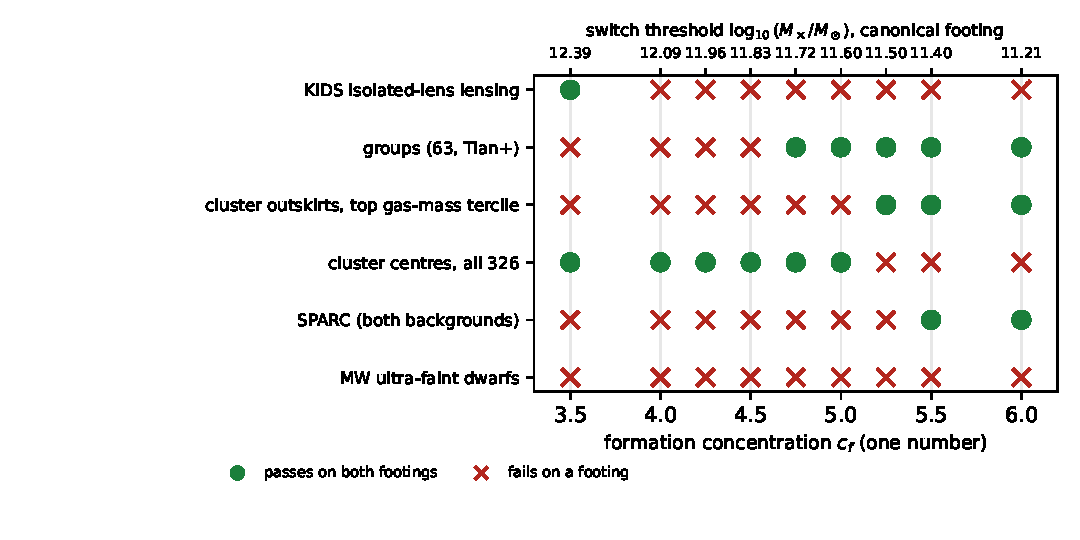
\includegraphics[width=0.92\linewidth]{PAPER63_fig_cfmap.pdf}\end{center}

Grid values at which each line passes on both footings: lensing 3.5 only; groups $\ge4.75$; cluster outskirts (top gas-mass tercile, G-OUT-M3) $\ge5.25$; cluster centres (G-IN-Mall) $\le5.0$; SPARC $\ge5.5$ (the alternative footing fails it below); the Milky Way ultra-faint dwarfs never pass on the alternative footing ($Z=-2.77$ at every $c_f$, a dwarf-side problem).

Two tensions follow, and they are the content of this note.
\begin{enumerate}
\item \textbf{Threshold against concentration.} The isolated KiDS lenses must carry no halo, so the threshold must sit at or above $\approx10^{12.4}\,M_\odot$ (canonical); groups need the concentration $c_f\ge4.75$. In the crossover construction a higher $c_f$ lowers the threshold, so the threshold cannot be the crossover. It must be set by something independent of halo concentration.
\item \textbf{Cluster inner against outer.} The outskirts want more concentration than the centres allow. GC1 (below) and the record's IB1 point the same way: the cluster halo's outer budget and its core concentration are separate degrees of freedom.
\end{enumerate}

\section{The outskirt deficit is inside turnaround (GC1)}
Every tested core rule leaves G-OUT-M3 under-predicted (X43 $c_f=4$: $Z=+2.41$; X38: $+5.4$; IB1 with the hydrostatic gas mass: $+5.02$). GC1 tested whether this is projected correlated structure beyond each cluster's turnaround radius, with zero free parameters (the record's CLASS linear correlation function and Mo--White bias, median $b=4.1$). The term changes the outer predictions by at most 1.3\,\% (G-OUT-M3 by 0.000): mass beyond turnaround projects as a nearly flat sheet, which carries no tangential shear. Moving the cluster normalisation to the native background (5.2715 for 5.364) makes G-OUT-M3 slightly worse ($+2.55$). Verdict: \textbf{NOT REPAIRED}, robust. The missing outer mass is inside turnaround.

\section{Below the threshold: the exclusion mechanism (M6)}
The surviving candidate for keeping cold dark energy out of galaxies below the threshold is M6: galaxies form in initial patches depleted of cold dark energy and enriched in baryons (compensated). Its decisive probe is the Lyman-$\alpha$ forest. Four framework-native forest models were frozen and run against Boera et al.\ (2019) and DESI DR1:
\begin{itemize}
\item P1D1 (linear proxy, $z$ 4.2--5.0) and P1D3 (linear proxy, DESI $z$ 2.2--4.4): not diagnostic (null $\chi^2$ 137.6/39 and 7017/719).
\item P1D2 (lognormal and saturation, $z$ 4.2--5.0): not diagnostic; saturation hides M6 there (Asimov $\Delta\chi^2$ 0.44 / 0.16).
\item P1D4 (3D lognormal with redshift-space distortion, DESI): not diagnostic (null $\chi^2$ 1864/690); the $z\ge3.6$ subset reaches 433/327.
\end{itemize}
In the regimes closest to adequate, M6 at X57's bound sits at the 95\,\% edge (P1D1 $k\le0.1$\,s/km: $\mu_{95}=1.26$; P1D3 $z\ge3.6$: $\mu_{95}=1.03$). M6N1 adds a derived requirement: with no exchange (X54) and X22's cap, a galaxy needing M6 must have at least 83.5\,\% (canonical) / 97.7\,\% (alternative) of its baryons patch-born. At the record's own Lagrangian retention (19.1\,\% / 16.3\,\%) M6 then needs more patch baryons than X57's provisional budget allows; it fits only if those galaxies retained at least 19--56\,\% (canonical) or 28--83\,\% (alternative) of their patch baryons.

\section{The question, stated precisely}
\begin{enumerate}
\item What physics switches cold dark energy on at $M\gtrsim10^{12.4}\,M_\odot$ (canonical footing), independently of the concentration of the halos it then forms? Candidates must leave isolated $L_\star$ systems (including the KiDS lenses) halo-free and give groups halos.
\item What sets a cluster's outer cold dark energy budget separately from its core concentration?
\item Below the threshold, how is cold dark energy kept out of galaxies? If by M6, what native forest model decides it, and do galaxies retain the required fraction of their patch baryons?
\end{enumerate}
What would decide them: a native threshold derivation compared with the CF1 map; converged native zoom concentrations (the ng\,64 runs are in progress) for the core side; a per-cent-level native forest model for M6.

\section*{Provenance}
Lane folders (repository \texttt{rebuild\_2026\_10\_22/}): CF1\_cf\_window\_map (criteria ef5a07c251, result e370b35e1c), GC1\_group\_cluster\_core\_rule (d1da6b8185, 09280e4b66), M6N1\_minimum\_patch\_need (3a2f5ca3a0, 3ab6a1bf44), P1D1--P1D4 (8f6e3db4bc, d50412913d, d89e0f9469, f05be7280b), X43, X58, X62. Every number above is checked against the committed lane outputs by \texttt{PAPER63\_audit.py}. AI assistance: Anthropic's Claude (analysis lanes, review, drafting).
\end{document}
